\documentclass[tikz,border=2pt]{standalone}
\usepackage{amsmath}
\usetikzlibrary{arrows.meta}
\begin{document}
% Call tree of Fibonacci(5): direct recursion makes 15 calls. With a cache the 6 calls F_5,...,F_0 on the
% left spine compute (blue), 3 calls are cache lookups (orange: F_1, F_2, F_3) and 6 calls are never made (grey).
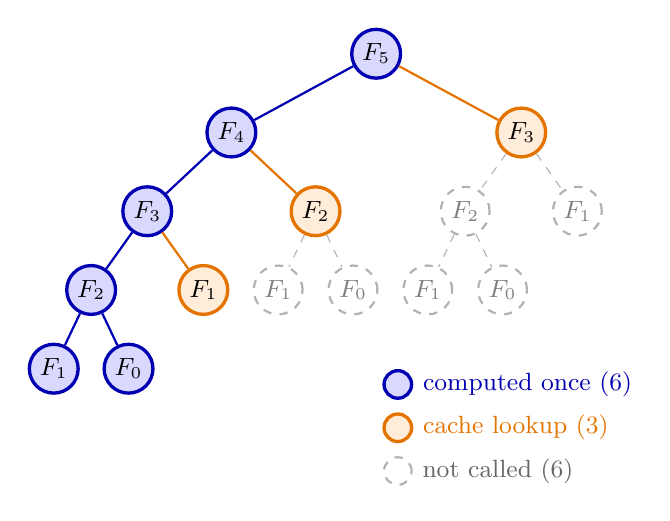
\begin{tikzpicture}[font=\small, >={Latex[length=2mm]}, x=0.95cm, y=-1.0cm,
  comp/.style={circle, draw=blue!70!black, very thick, fill=blue!15, inner sep=1.5pt, minimum size=0.62cm},
  look/.style={circle, draw=orange!90!black, very thick, fill=orange!15, inner sep=1.5pt, minimum size=0.62cm},
  skip/.style={circle, draw=gray!60, dashed, thick, text=gray, inner sep=1.5pt, minimum size=0.62cm}]
  % computed spine
  \node[comp] (f5) at (4.31,0) {$F_5$};
  \node[comp] (f4) at (2.375,1) {$F_4$};
  \node[comp] (f3a) at (1.25,2) {$F_3$};
  \node[comp] (f2a) at (0.5,3) {$F_2$};
  \node[comp] (f1a) at (0,4) {$F_1$};
  \node[comp] (f0a) at (1,4) {$F_0$};
  % cache lookups
  \node[look] (f1b) at (2,3) {$F_1$};
  \node[look] (f2b) at (3.5,2) {$F_2$};
  \node[look] (f3b) at (6.25,1) {$F_3$};
  % calls that are never made with the cache
  \node[skip] (f1c) at (3,3) {$F_1$};
  \node[skip] (f0c) at (4,3) {$F_0$};
  \node[skip] (f2c) at (5.5,2) {$F_2$};
  \node[skip] (f1d) at (7,2) {$F_1$};
  \node[skip] (f1e) at (5,3) {$F_1$};
  \node[skip] (f0e) at (6,3) {$F_0$};
  \draw[thick, blue!70!black] (f5) -- (f4) (f4) -- (f3a) (f3a) -- (f2a) (f2a) -- (f1a) (f2a) -- (f0a);
  \draw[thick, orange!90!black] (f5) -- (f3b) (f4) -- (f2b) (f3a) -- (f1b);
  \draw[thin, dashed, gray!60] (f2b) -- (f1c) (f2b) -- (f0c) (f3b) -- (f2c) (f3b) -- (f1d)
    (f2c) -- (f1e) (f2c) -- (f0e);
  % short legend
  \node[comp, minimum size=0.35cm, label={[blue!70!black]east:computed once (6)}] at (4.6,4.2) {};
  \node[look, minimum size=0.35cm, label={[orange!90!black]east:cache lookup (3)}] at (4.6,4.75) {};
  \node[skip, minimum size=0.35cm, label={[gray!80!black]east:not called (6)}] at (4.6,5.3) {};
\end{tikzpicture}
\end{document}
